\chapter{Resultados}
\label{chap:resultados}


\drop{A} lo largo de este capítulo, se desarrolla los resultados obtenidos según la evolución en cada uno de los aspectos de la plataforma de juego.
\begin{itemize}
\item Estructura de la aplicación.
\item Comunicaciones cliente-servidor.
\item Sistema de localización.
\item Lectura, tratamiento y comunicación de datos, de los sensores.
\item Gestión de eventos de la aplicación. Máquina de estados.
\item Diseño software de la interfaz gráfica.
\item Actualización software de la aplicación.
\end{itemize}


\section{Estructura de la aplicación.}
El funcionamiento de los dispositivos \emph{TUIO1} y \emph{TUIO1} es gestionado con el uso de \emph{Maquinas de Estado Finitos (FSM)}\footnote{Finite State Machine.}.


\subsection{Máquina de estados finitos dispositivo TUIO1.}

\begin{itemize}
\item \textbf{IDLE:} Estado inicial del dispositivo \emph{TUIO1}. La máquina permanece en este estado hasta recibir confirmación de comunicación con el dispositivo \emph{TUIO2}.\\
\textbf{Transiciones/eventos.}
\begin{itemize}
\item \texttt{tuio2\_connect:} transición de estado \textbf{IDLE} a \textbf{MAIN} cuando se establece las comunicaciones cliente-servidor.
\item \texttt{exit\_tuio1:} transición de estado \textbf{IDLE} a \textbf{EXIT} al recibir el evento salir de la aplicación.
\item \texttt{init\_server:} evento interno para iniciar el servidor.
\end{itemize}


\item \textbf{MAIN:} Estado principal de la aplicación una vez establecida la comunicación entre los dispositivos \emph{TUIO1} y \emph{TUIO2}.\\
\textbf{Transiciones/eventos.}
\begin{itemize}
\item \texttt{tuio2\_disconnect:} transición desde el estado \textbf{MAIN} a \textbf{IDLE} cuando se han perdido las comunicaciones con \emph{TUIO2}.
\item \texttt{start\_game:} transición desde el estado \textbf{MAIN} a \textbf{GAME}, al recibir el evento de comenzar el juego.
\item \texttt{exit\_tuio1:} transición de estado \textbf{IDLE} a \textbf{EXIT} al recibir el evento salir de la aplicación.
\end{itemize}


\item \textbf{GAME:} El dispositivo comienza a ejecutar el juego. Se crea un evento de salida para el dispositivo \emph{TUIO2}, el cual recibe la orden de cambiar su estado a \textbf{GAME}.\\
\textbf{Transiciones/eventos.}
\begin{itemize}
\item \texttt{stop\_game:} transición desde el estado \textbf{GAME} a \textbf{MAIN} al recibir el evento de finalizar el juego.
\item \texttt{tuio2\_disconnect:} transición desde el estado \textbf{GAME} a \textbf{IDLE} cuando se han perdido las comunicaciones con \emph{TUIO2}.
\item \texttt{exit\_tuio1:} transición de estado \textbf{GAME} a \textbf{EXIT} al recibir el evento salir de la aplicación.
\item \texttt{request\_data:} evento de salida para solicitar datos al dispositivo \emph{TUIO2}.
\item \texttt{receive\_data:} evento de entrada al recibir datos desde el dispositivo \emph{TUIO2}.
\end{itemize}


\item \textbf{EXIT:} Estado de la máquina por el cual se finaliza toda la aplicación.\\
\textbf{Eventos.}
\begin{itemize}
\item \texttt{exit\_tuio1:} evento de entrada para finalizar la ejecución de la aplicación.
\end{itemize}
\end{itemize}

La Figura ~\ref{fig:tuio1fsmv0} muestra la estructura de la máquina de estados del dispositivo \emph{TUIO1}

\begin{figure}[!h]
\begin{center}
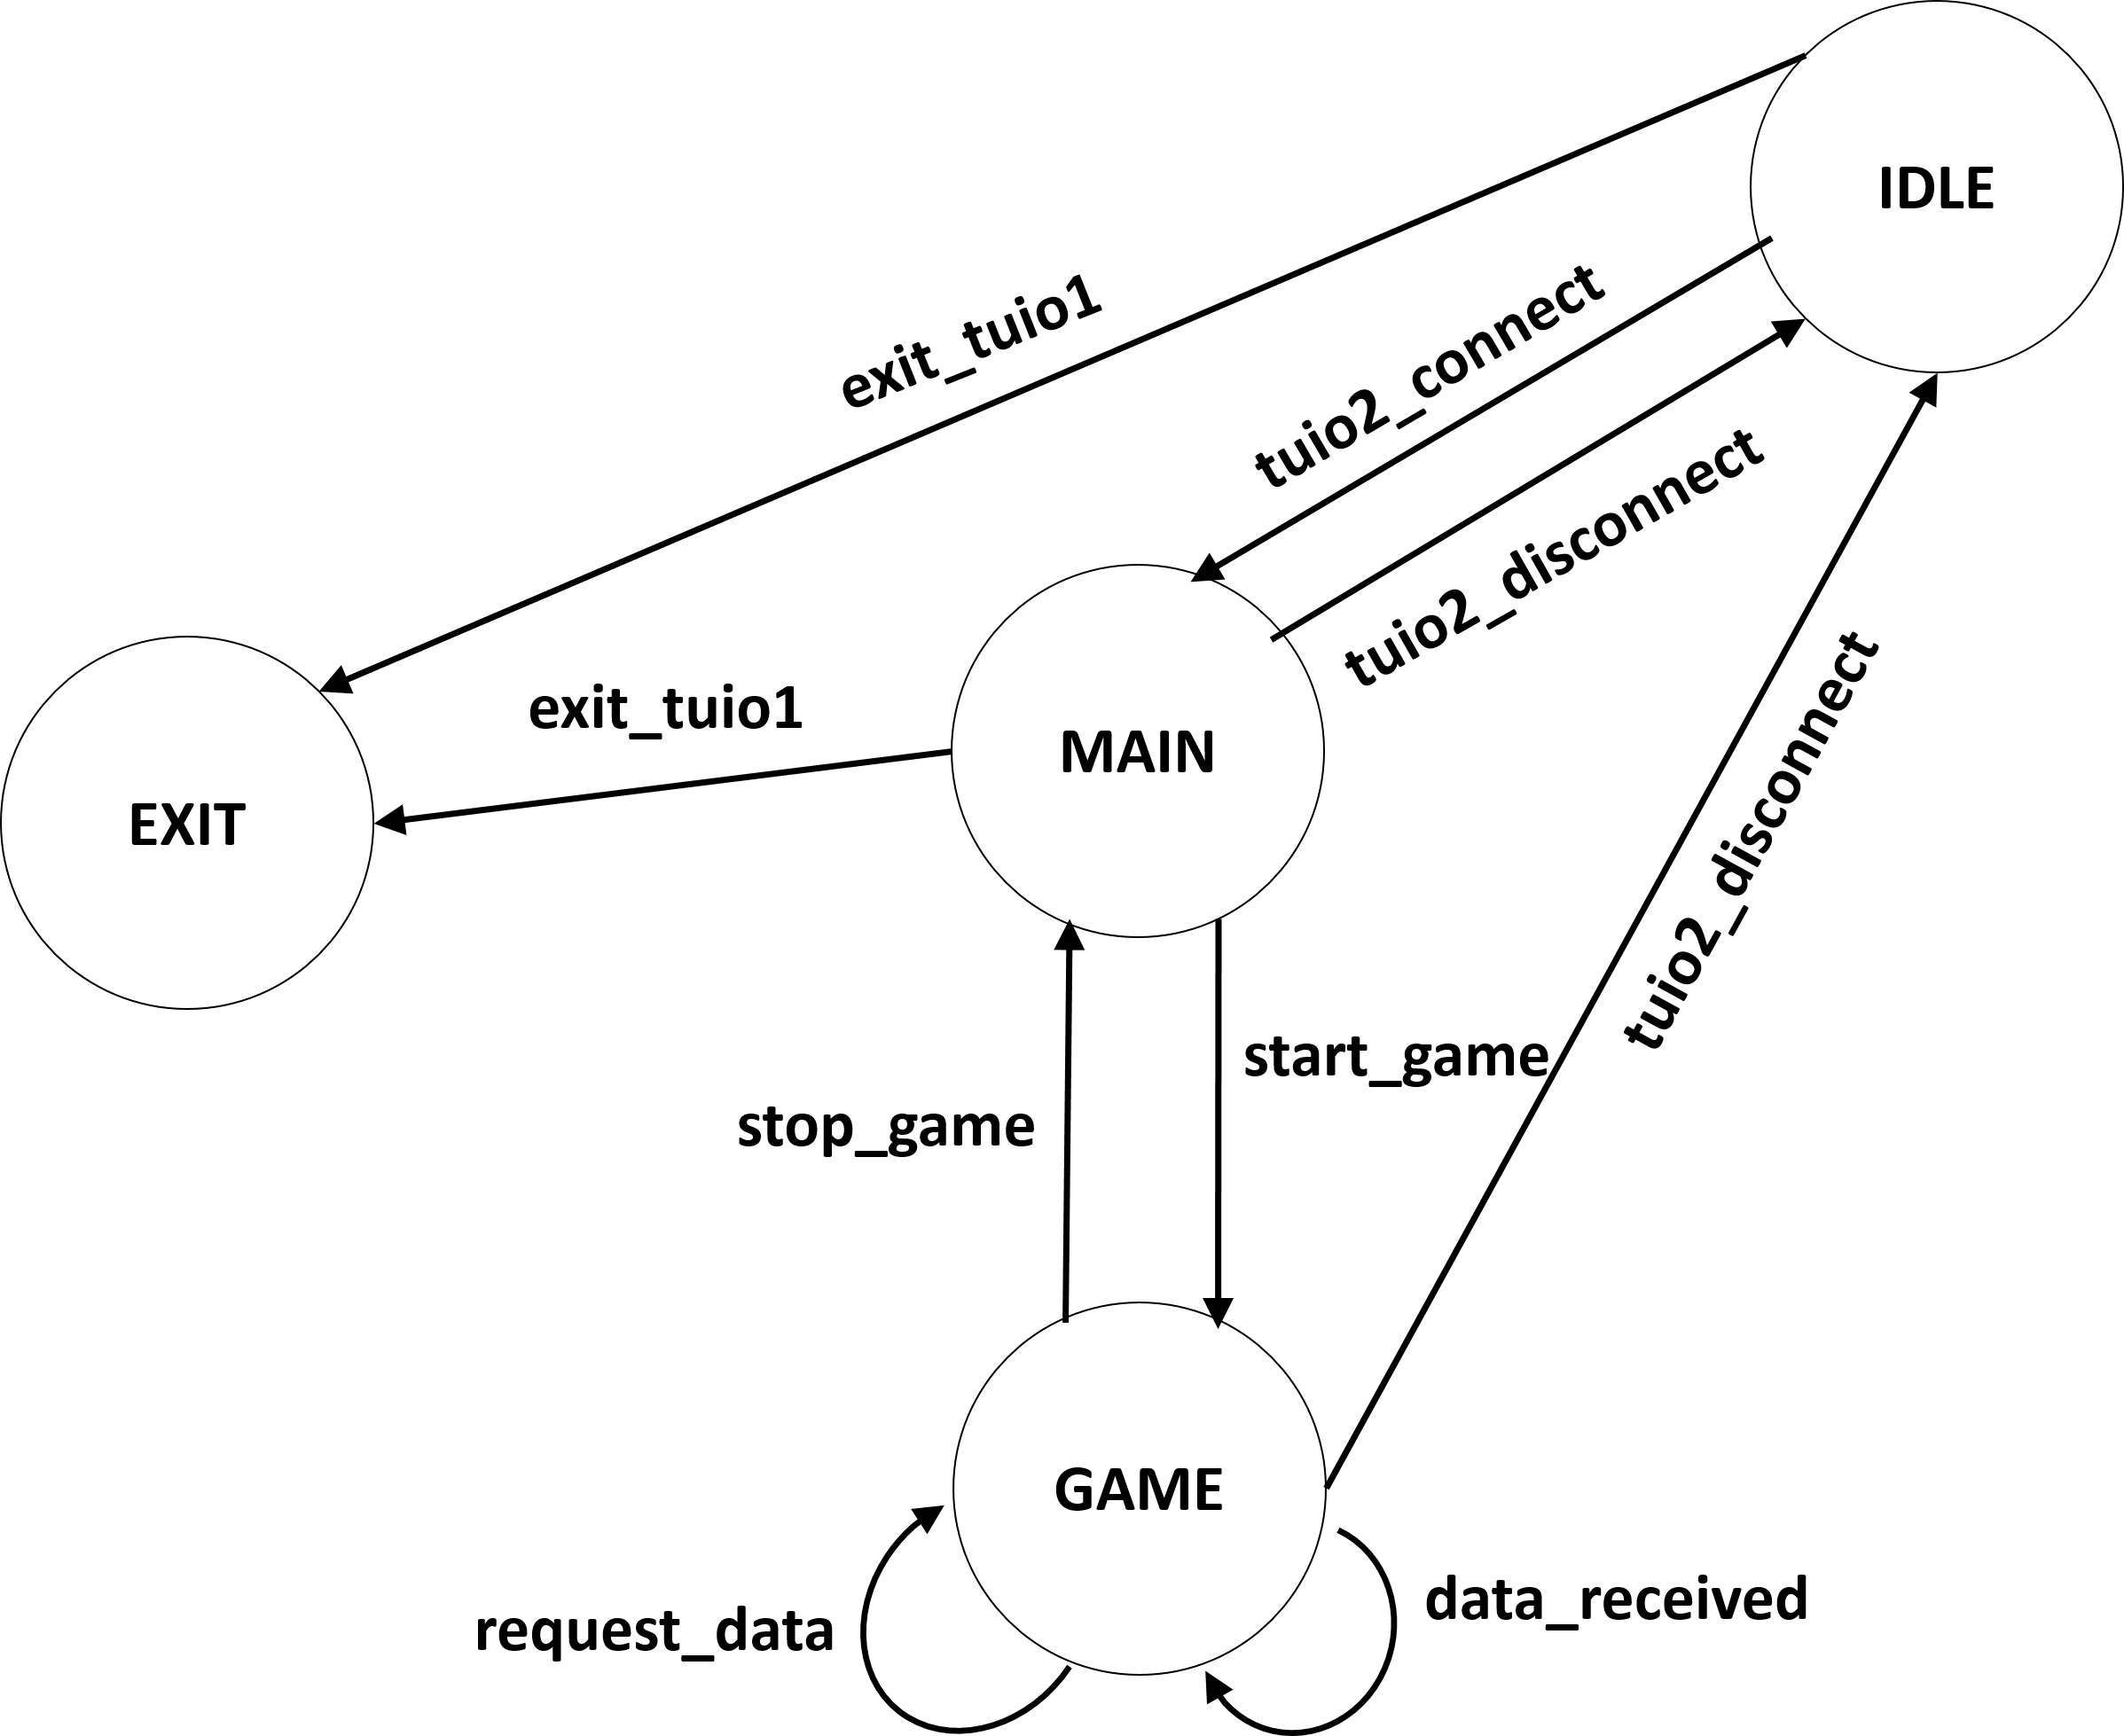
\includegraphics[width=0.7\textwidth]{fsm_tuio1_v0.png}
\caption{Estructura máquina de estados finitos TUIO1 (versión pruebas).}
\label{fig:tuio1fsmv0}
\end{center}
\end{figure}



\subsection{Máquina de estados finitos Servidor.}

\begin{itemize}
\item \textbf{IDLE:} Estado inicial del servidor a la espera de recibir un evento desde la máquina de estados del dispositivo \emph{TUIO1} para iniciar el servidor. Dispone de dos transiciones de estado posible, y tres eventos de entrada.\\
\textbf{Transiciones/Eventos.}
\begin{itemize}
\item \texttt{init\_server:} transición al estado \textbf{LISTEN}. La ejecución de esta transición sucede cuando la máquina de estados del servidor recibe el evento \texttt{init\_server} dentro de la máquina de estados \texttt{ServerFSM}. El evento puede ser creado por tres posibles entradas.
\item \texttt{close\_server:} transición al estado \textbf{EXIT} al recibir el evento \texttt{close\_server} desde la máquina de estados \texttt{Tuio1FSM}, para cerrar el servidor.\\
\item \texttt{create\_server}. Entrada desde la máquina de estados \texttt{Tuio1FSM}, al iniciar el dispositivo.
\item \texttt{reconnect}(perdida de conexión). Entrada de evento de reconexión al interrumpirse la conexión con el cliente \emph{(TUIO2)}.
\item \texttt{reconnect}(tiempo de espera). Agotado tiempo de espera para conectar con \emph{TUIO2}.
\end{itemize}


\item \textbf{LISTEN:} El servidor queda a la espera de conectar con el cliente (\emph{TUIO2}). En el caso de no conectar con el cliente (en un tiempo definido de 10 segundos), es ejecutada la transición \texttt{reconnect}. 
Al conectar con \emph{TUIO2} (cliente), \emph{ServerFSM} ejecuta la transición \texttt{wait\_data} hasta el estado \textbf{CONNECT}, a la espera de recibir datos desde \emph{TUIO2}. Al establecer la conexión con el cliente, se crea un evento de entrada indicando que las comunicaciones han sido establecidas.
\textbf{Transiciones.}
\begin{itemize}
\item \texttt{reconnect}: la máquina vuelve al estado \textbf{IDLE}, al agotarse el tiempo de espera para conectar con el cliente. Se crea el evento \emph{init\_server}, para volver a iniciar el servidor.\\
\item \texttt{close\_server:} transición al estado \textbf{EXIT} al recibir el evento \texttt{close\_server} desde la máquina de estados \texttt{Tuio1FSM}, para cerrar el servidor.\\
\textbf{Entradas.}
\item \texttt{init\_server:} el servidor queda a la espera de conectar con el cliente \emph{TUIO2}.
\end{itemize}


\item \textbf{CONNECT:} Existe comunicación entre los dispositivos \emph{TUIO1} y \emph{TUIO2}. 
Dispone de dos entradas y una transición posible: recibir datos, enviar datos, o volver a iniciar el servidor si la conexión ha sido interrumpida respectivamente.\\
\textbf{Transiciones.}
\begin{itemize}
\item \texttt{reconnect}: la máquina vuelve al estado \textbf{IDLE}, al interrumpirse la comunicación con el cliente. Se crea el evento \emph{init\_server}, para volver a iniciar el servidor.
\item \texttt{close\_server:} transición al estado \textbf{EXIT} al recibir el evento \texttt{close\_server} desde la máquina de estados \texttt{Tuio1FSM}, para cerrar el servidor.\\
\textbf{Entradas.}
\item \texttt{receive\_data} es ejecutada si se reciben datos desde \emph{TUIO2}. Los datos son añadidos a una lista (cola), la cual es manejada por \emph{Tuio1FSM} (por medio de \texttt{data\_received}). Se mantiene en el estado \textbf{CONNECT}, a la espera de recibir mas datos desde \emph{TUIO2}.
\item \texttt{send\_data:} envia datos al cliente \texttt{TUIO2}.
\end{itemize}


\item \textbf{EXIT:} Estado de la máquina por el cual se finaliza el servidor.\\
\textbf{Eventos.}
\begin{itemize}
\item \texttt{close\_server:} evento de entrada para finalizar la ejecución del servidor.
\end{itemize}
\end{itemize}

La Figura ~\ref{fig:fsmserverv0} muestra la estructura de la máquina de estados del dispositivo \emph{TUIO2}

\begin{figure}[!h]
\begin{center}
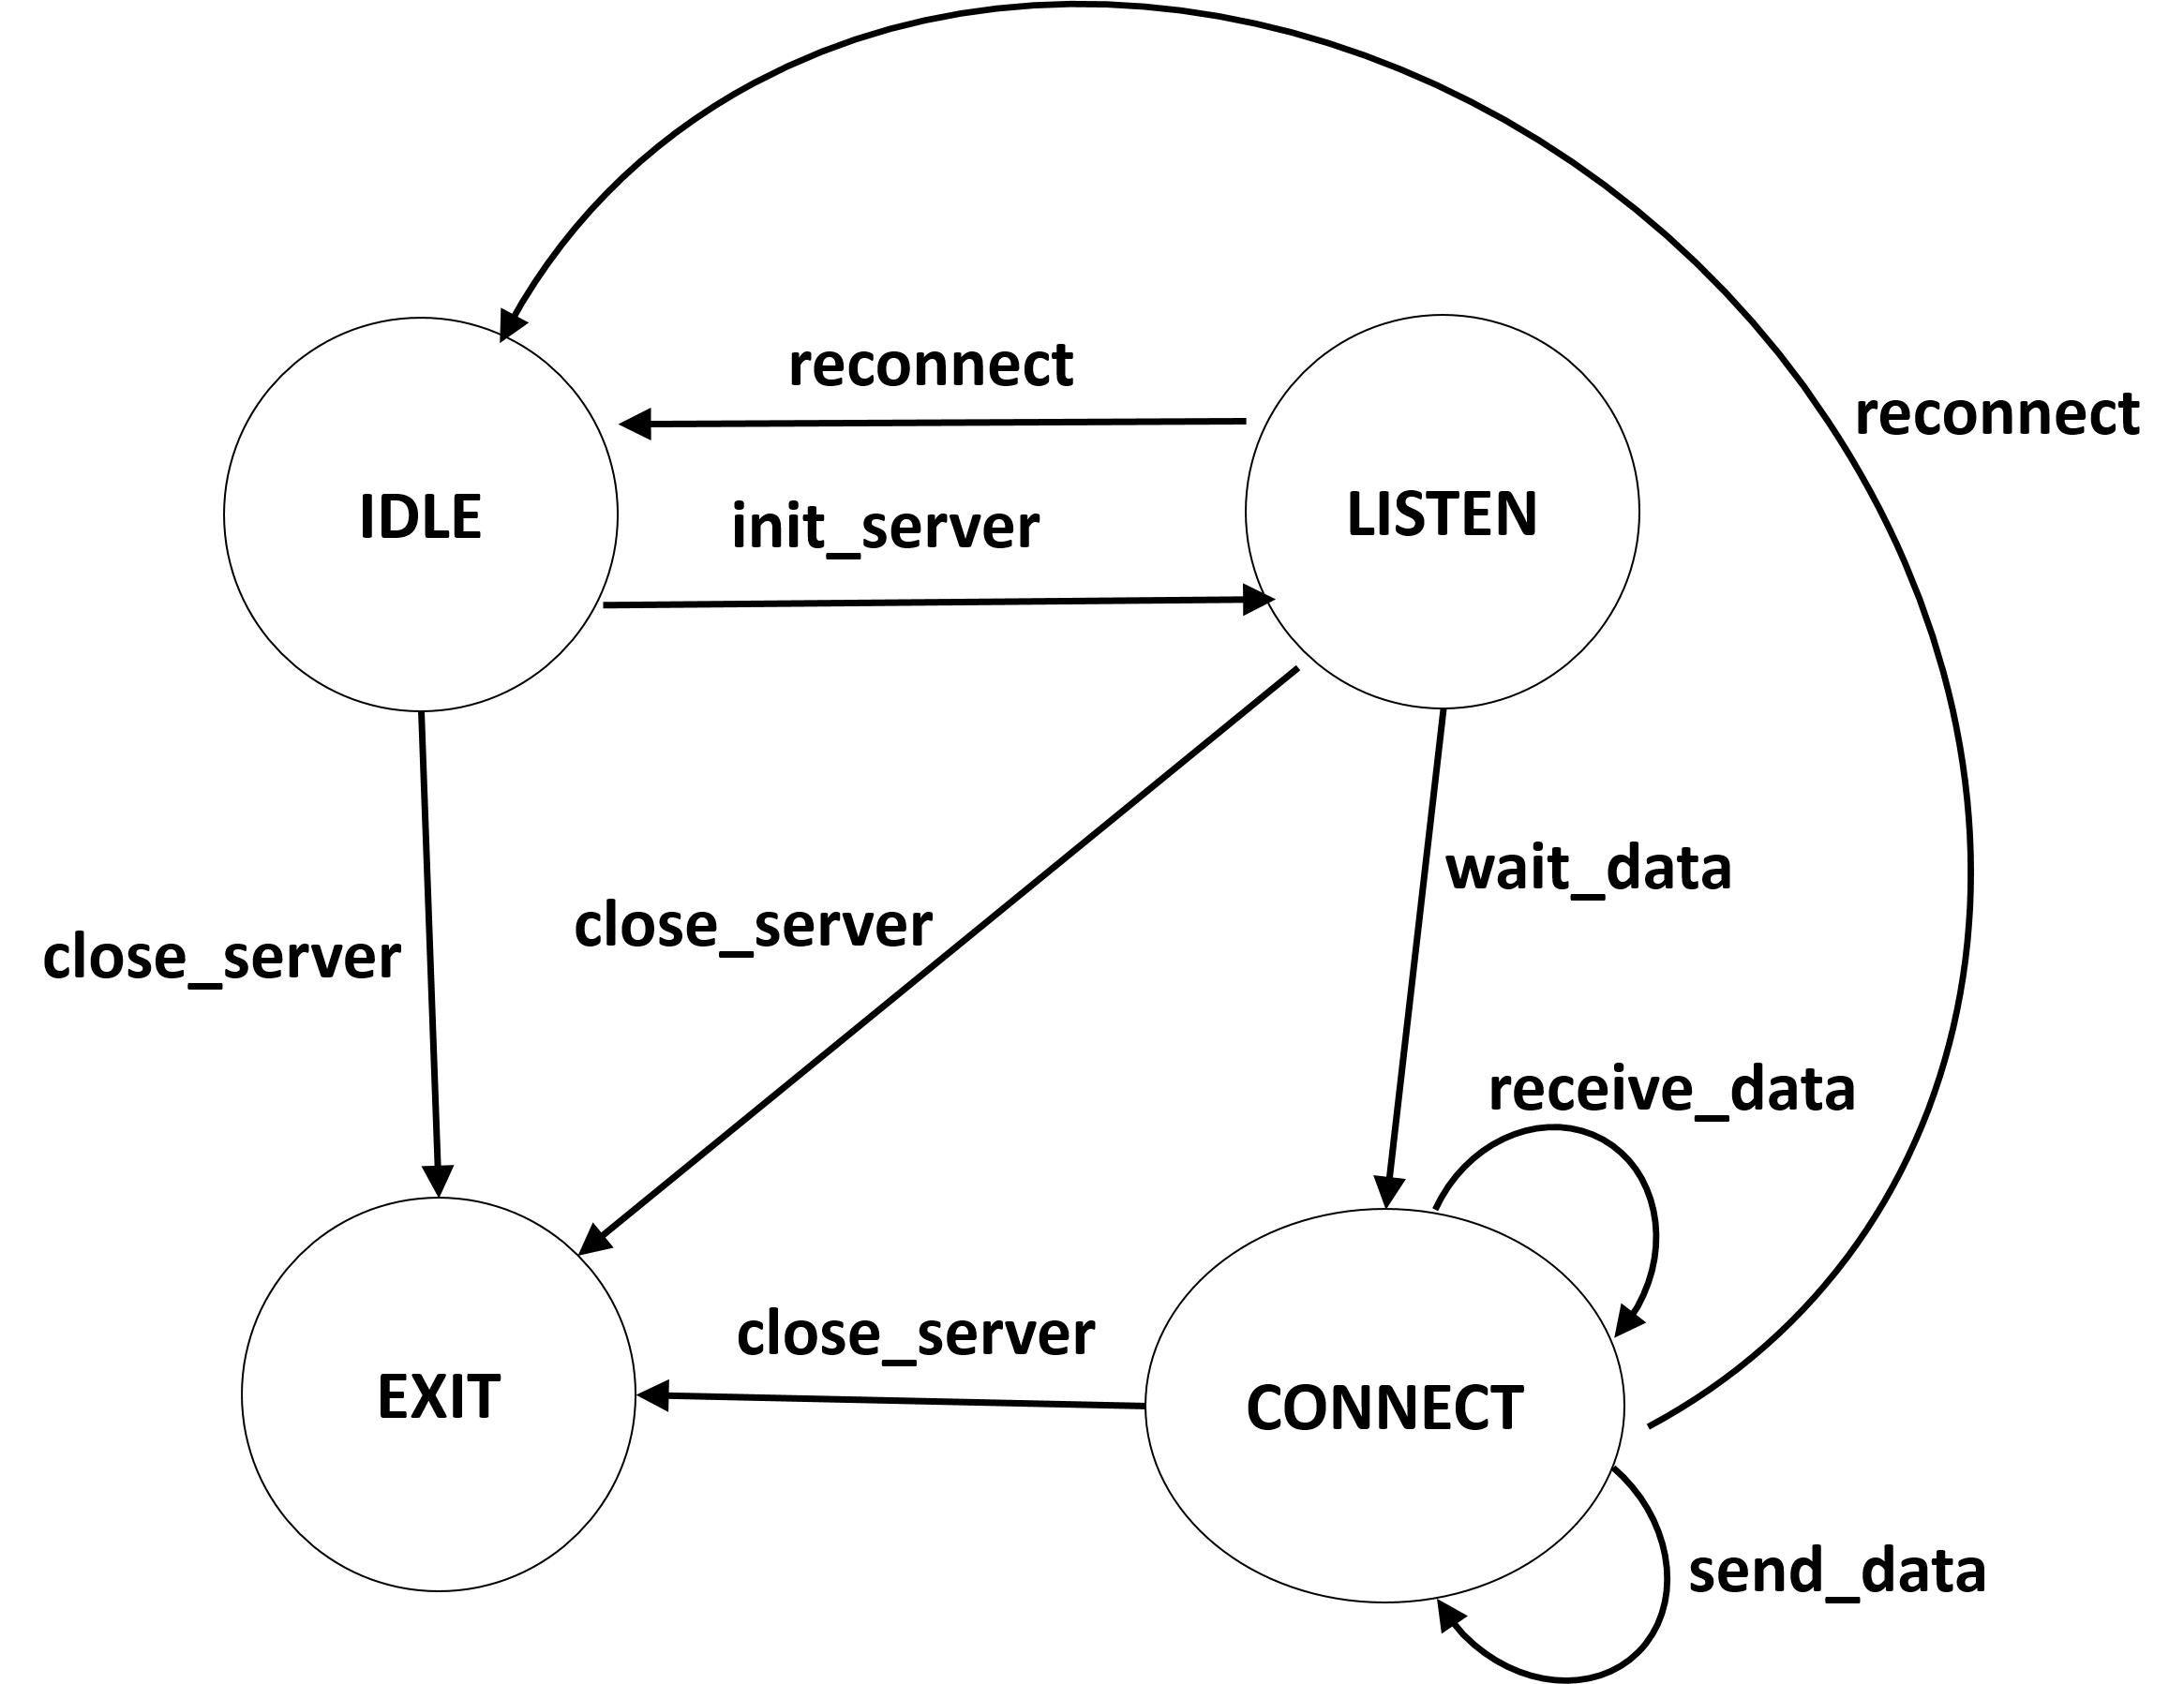
\includegraphics[width=0.7\textwidth]{fsm_server_v0.png}
\caption{Estructura máquina de estados finitos del servidor (versión pruebas).}
\label{fig:fsmserverv0}
\end{center}
\end{figure}




\subsection{Máquina de estados finitos dispositivo TUIO2.}

\begin{itemize}
\item \textbf{IDLE:} Estado inicial del dispositivo \emph{TUIO2}. La máquina permanece en este estado hasta recibir confirmación de comunicación con el dispositivo \emph{TUIO1}.\\
\textbf{Transiciones/eventos.}
\begin{itemize}
\item \texttt{tuio1\_connect:} transición de estado \textbf{IDLE} a \textbf{MAIN} cuando se establece las comunicaciones cliente-servidor.
\item \texttt{exit\_tuio2:} transición de estado \textbf{IDLE} a \textbf{EXIT} al recibir el evento salir de la aplicación.
\item \texttt{init\_client:} evento interno para iniciar el cliente.
\end{itemize}


\item \textbf{MAIN:} Estado principal de la aplicación una vez establecida la comunicación entre los dispositivos \emph{TUIO1} y \emph{TUIO2}.\\
\textbf{Transiciones/eventos.}
\begin{itemize}
\item \texttt{tuio1\_disconnect:} transición desde el estado \textbf{MAIN} a \textbf{IDLE} cuando se han perdido las comunicaciones con \emph{TUIO1}.
\item \texttt{start\_game:} transición desde el estado \textbf{MAIN} a \textbf{GAME}, al recibir el evento de comenzar el juego.
\item \texttt{exit\_tuio2:} transición de estado \textbf{IDLE} a \textbf{EXIT} al recibir el evento salir de la aplicación.
\end{itemize}


\item \textbf{GAME:} El dispositivo comienza a ejecutar el juego al recibir un evento desde el dispositivo \emph{TUIO1}, el cual envía la orden de cambiar el estado a \textbf{GAME}.\\
\textbf{Transiciones/eventos.}
\begin{itemize}
\item \texttt{stop\_game}: transición desde el estado \textbf{GAME} a \textbf{MAIN} al recibir el evento de finalizar el juego.
\item \texttt{tuio1\_disconnect}: transición desde el estado \textbf{GAME} a \textbf{IDLE} cuando se han perdido las comunicaciones con \emph{TUIO1}.
\item \texttt{exit\_tuio2:} transición de estado \textbf{GAME} a \textbf{EXIT} al recibir el evento salir de la aplicación.
\item \texttt{send\_data}: evento de salida para enviar datos al dispositivo \emph{TUIO1}.
\item \texttt{data\_treatment}: evento de entrada para tratar datos/eventos recibidos desde el dispositivo \emph{TUIO1}.
\end{itemize}


\item \textbf{EXIT:} Estado de la máquina por el cual se finaliza toda la aplicación.\\
\textbf{Eventos.}
\begin{itemize}
\item \texttt{exit\_tuio2:} evento de entrada para finalizar la ejecución de la aplicación.
\end{itemize}
\end{itemize}

La Figura ~\ref{fig:tuio2fsmv0} muestra la estructura de la máquina de estados del dispositivo \emph{TUIO2}

\begin{figure}[!h]
\begin{center}
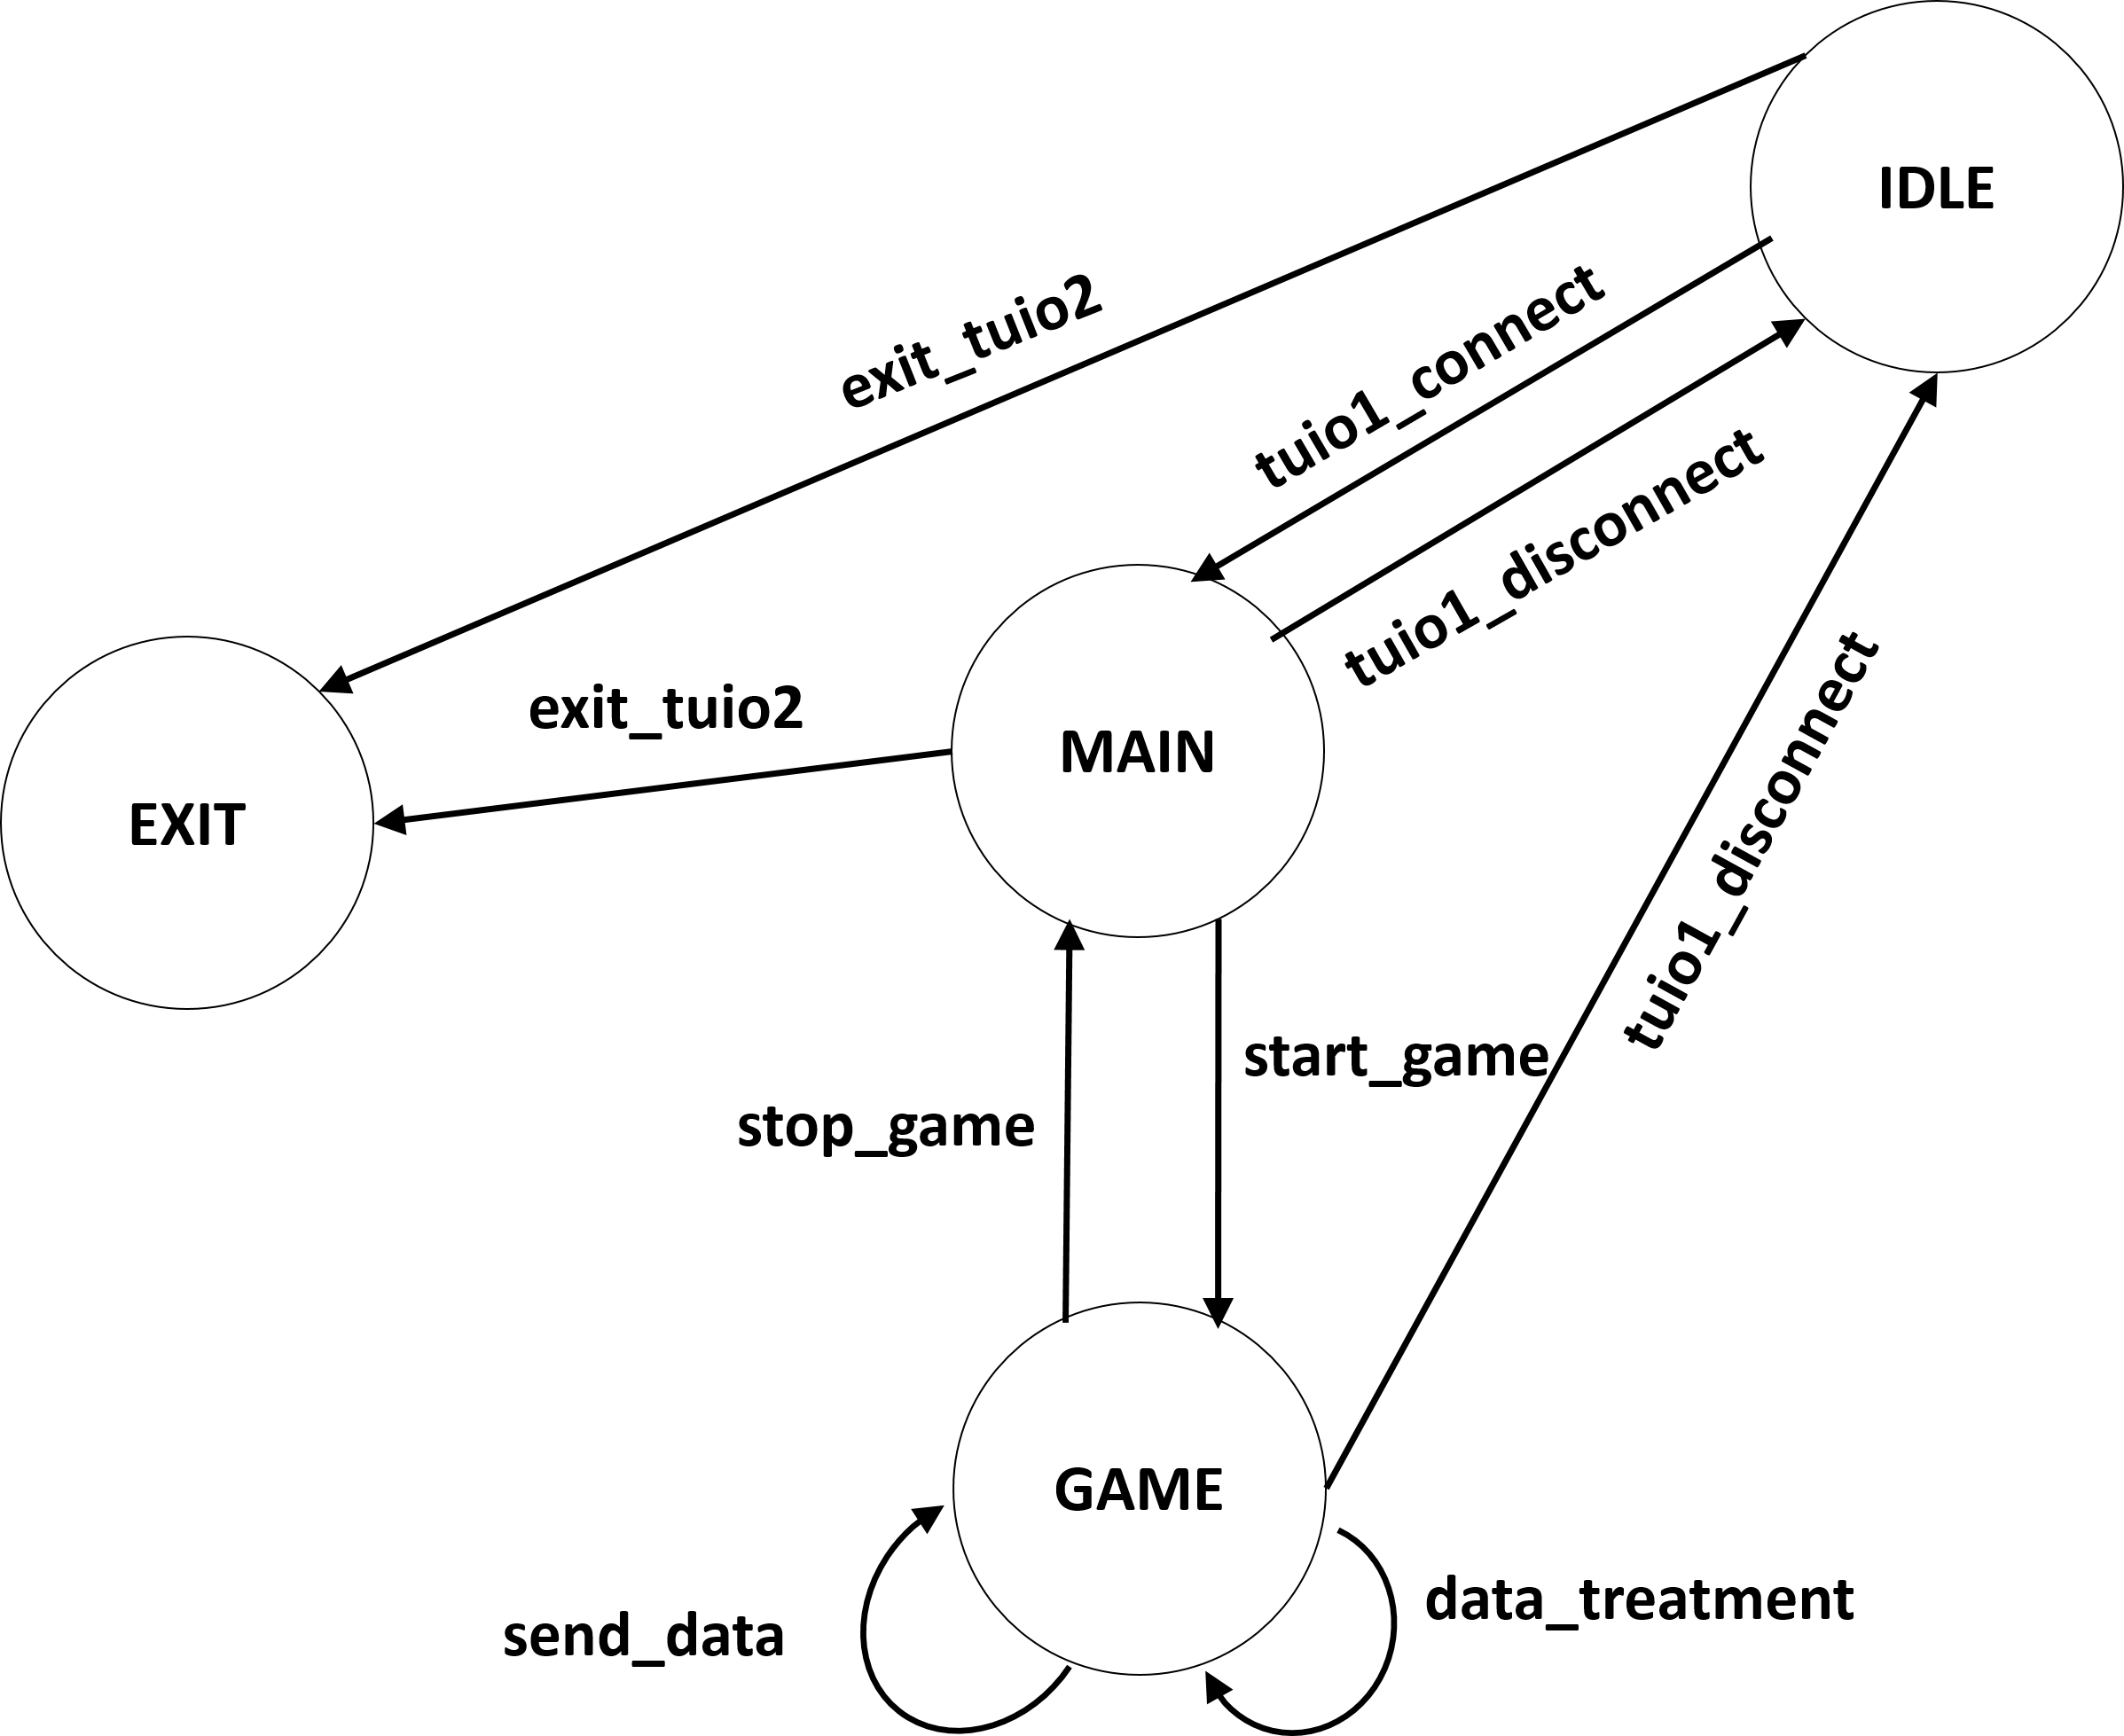
\includegraphics[width=0.7\textwidth]{fsm_tuio2_v0.png}
\caption{Estructura máquina de estados finitos TUIO2 (versión pruebas).}
\label{fig:tuio2fsmv0}
\end{center}
\end{figure}


\subsection{Máquina estados finitos Cliente.}

\begin{itemize}
\item \textbf{IDLE:} Estado inicial del cliente a la espera de recibir un evento desde la máquina de estados del dispositivo \emph{TUIO2} para iniciar el cliente. Dispone de dos transiciones de estado posible, y tres eventos de entrada.\\
\textbf{Transiciones/Eventos.}
\begin{itemize}
\item \texttt{init\_cliente:} transición al estado \textbf{LISTEN}. La ejecución de esta transición sucede cuando la máquina de estados del cliente recibe el evento \texttt{init\_cliente} dentro de la máquina de estados \texttt{ClientFSM}. El evento puede ser creado por tres posibles entradas.
\item \texttt{close\_client:} transición al estado \textbf{EXIT} al recibir el evento \texttt{close\_cliente} desde la máquina de estados \texttt{Tuio2FSM}, para cerrar el cliente.\\
\item \texttt{create\_client}. Entrada desde la máquina de estados \texttt{Tuio2FSM}, al iniciar el dispositivo.
\item \texttt{reconnect}(perdida de conexión). Entrada de evento de reconexión al interrumpirse la conexión con el servidor \emph{(TUIO1)}.
\item \texttt{reconnect}(tiempo de espera). Agotado tiempo de espera para conectar con \emph{TUIO1}.
\end{itemize}


\item \textbf{LISTEN:} El servidor queda a la espera de conectar con el servidor (\emph{TUIO1}). En el caso de no conectar con el servidor (en un tiempo definido de 10 segundos), es ejecutada la transición \texttt{reconnect}. 
Al conectar con \emph{TUIO1} (servidor), \emph{ClientFSM} ejecuta la transición \texttt{wait\_data} hasta el estado \textbf{CONNECT}, a la espera de recibir datos desde \emph{TUIO1}. Al establecer la conexión con el servidor, se crea un evento de entrada indicando que las comunicaciones han sido establecidas.
\textbf{Transiciones.}
\begin{itemize}
\item \texttt{reconnect}: la máquina vuelve al estado \textbf{IDLE}, al agotarse el tiempo de espera para conectar con el servidor. Se crea el evento \emph{init\_client}, para volver reestablecer el cliente.\\
\item \texttt{close\_client:} transición al estado \textbf{EXIT} al recibir el evento \texttt{close\_client} desde la máquina de estados \texttt{Tuio2FSM}, para cerrar el cliente.\\
\textbf{Entradas.}
\item \texttt{init\_client:} el cliente queda a la espera de conectar con el servidor \emph{TUIO1}.
\end{itemize}


\item \textbf{CONNECT:} Existe comunicación entre los dispositivos \emph{TUIO1} y \emph{TUIO2}. 
Dispone de dos entradas y una transición posible: recibir datos, enviar datos, o volver a iniciar el cliente si la conexión ha sido interrumpida respectivamente.\\
\textbf{Transiciones.}
\begin{itemize}
\item \texttt{reconnect}: la máquina vuelve al estado \textbf{IDLE}, al interrumpirse la comunicación con el servidor. Se crea el evento \emph{init\_client}, para volver a iniciar el cliente.
\item \texttt{close\_client:} transición al estado \textbf{EXIT} al recibir el evento \texttt{close\_client} desde la máquina de estados \texttt{Tuio2FSM}, para cerrar el cliente.\\
\textbf{Entradas.}
\item \texttt{receive\_data} es ejecutada si se reciben datos desde \emph{TUIO1}. Los datos son añadidos a una lista (cola), la cual es manejada por \emph{Tuio2FSM} (por medio de \texttt{data\_treatment
}). Se mantiene en el estado \textbf{CONNECT}, a la espera de recibir mas datos desde \emph{TUIO1}.
\item \texttt{send\_data:} envía datos al servidor \texttt{TUIO1}.
\end{itemize}


\item \textbf{EXIT:} Estado de la máquina por el cual se finaliza el cliente.\\
\textbf{Eventos.}
\begin{itemize}
\item \texttt{close\_client:} evento de entrada para finalizar la ejecución del cliente.
\end{itemize}
\end{itemize}

La Figura ~\ref{fig:fsmclientv0} muestra la estructura de la máquina de estados del cliente.

\begin{figure}[!h]
\begin{center}
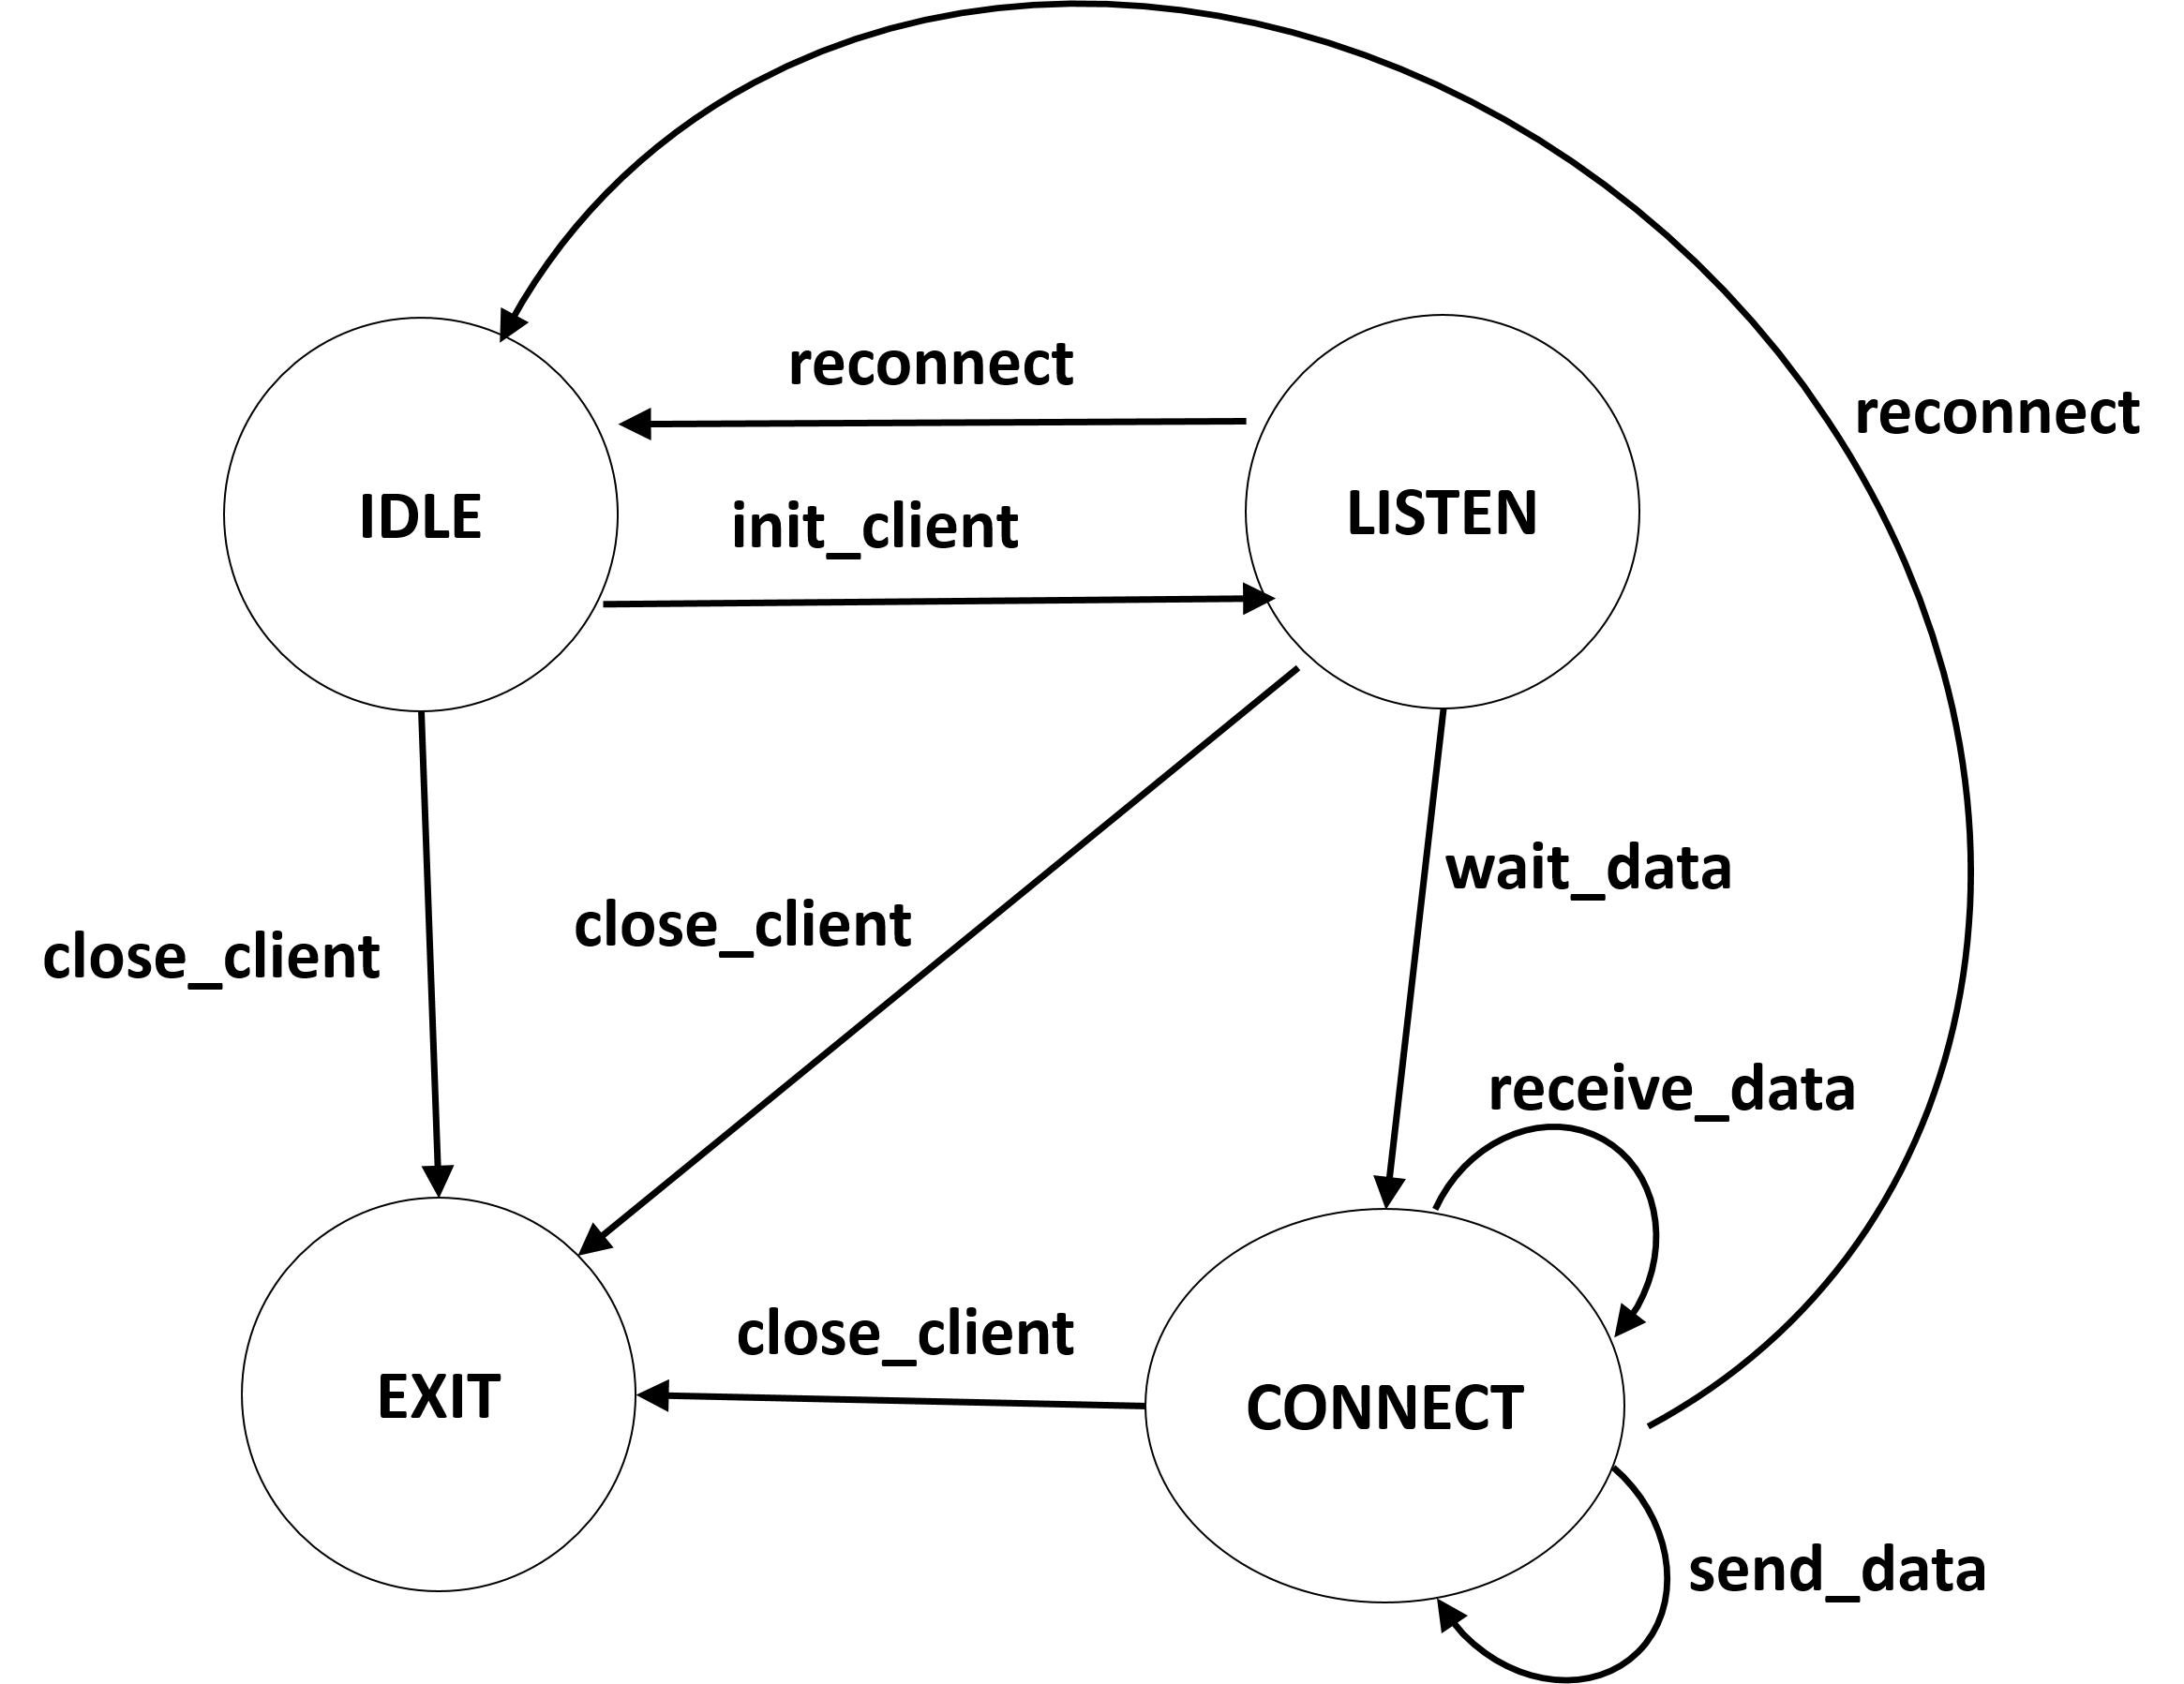
\includegraphics[width=0.7\textwidth]{fsm_client_v0.png}
\caption{Estructura máquina de estados finitos del cliente (versión pruebas).}
\label{fig:fsmclientv0}
\end{center}
\end{figure}

\section{Comunicaciones cliente-servidor.}
\label{sec:comunicaciones}
Siguiendo la estructura expuesta en la sección anterior, se escribe el código para crear las máquinas de estados finitos para ambos dispositivos.

Disposición de los archivos del dispositivo \emph{TUIO1:}
\begin{itemize}
\item Código principal y máquina de estados de la aplicación: \texttt{\textbackslash itanium\textbackslash Tuio1.py}
\item Código y máquina de estados del servidor: \texttt{\textbackslash itanium\textbackslash lib\textbackslash Server.py}
\end{itemize} 

Disposición de los archivos del dispositivo \emph{TUIO2:}
\begin{itemize}
\item Código principal y máquina de estados de la aplicación: \texttt{\textbackslash itanium\textbackslash Tuio2.py}
\item Código y máquina de estados del cliente: \texttt{\textbackslash itanium\textbackslash lib\textbackslash Client.py}
\item Código y máquina de estados del sensor \emph{MPU-9255}: \texttt{\textbackslash itanium\textbackslash lib\textbackslash MPU9255.py}
\end{itemize}

\subsection{Programa de pruebas de las comunicaciones cliente-servidor.}

El programa de pruebas consiste en realizar él envió/recepción de datos entre los dispositivos, donde se realizan secuencias básicas en las comunicaciones.
La secuencia que realiza el programa de pruebas en las comunicaciones cliente servidor, es la siguiente:

El servidor se inicia en el \emph{puerto 8888} y queda a la espera de la conexión del cliente. Se imprime por pantalla lado servidor: «Esperando cliente». 

Una vez el cliente establece la comunicación con el servidor, se imprime por pantalla en lado servidor: «Cliente conectado». De igual manera, en el lado cliente se imprime por pantalla: «Conectado a servidor».

Se crea un evento para indicar a ambos dispositivos que se inicie el juego (estado \textbf{GAME}). Se imprime por pantalla el mensaje: «Juego iniciado»

Cuando ambos dispositivos estén en el estado \textbf{GAME}, el servidor envía una petición de datos de la unidad de medición inercial \emph{MPU-9255}.

Este evento es gestionado en el programa principal \texttt{tuio2}, que devuelve la petición solicitada del servidor. Se imprime por pantalla: «Datos enviados al servidor.». Son mostrados los datos recibidos en el servidor, una vez manejado el evento de entrada: «Datos recibidos del cliente: » 

Finaliza la conexión y la aplicación de ambos dispositivos, mostrando respectivamente: «Aplicación finalizada»

La Figura ~\ref{fig:fsmexample} muestra de manera gráfica, la secuencia básica expuesta para las pruebas de las comunicaciones.

\begin{figure}[!h]
\begin{center}
\includegraphics[width=0.7\textwidth]{fsm_example.png}
\caption{Estructura de la secuencia de las pruebas cliente-servidor.}
\label{fig:fsmexample}
\end{center}
\end{figure}


\section{Sistema de localización.}

\section{Lectura, tratamiento y comunicación de datos, de los sensores.}

\section{Gestión de eventos de la aplicación. Máquina de estados.}

\section{Diseño software de la interfaz gráfica.}

\section{Actualización software de la aplicación.}




